\documentclass[]{article}
\usepackage{lmodern}
\usepackage{amssymb,amsmath}
\usepackage{ifxetex,ifluatex}
\usepackage{graphicx}
\usepackage[final]{pdfpages}
\usepackage{fixltx2e} % provides \textsubscript
\ifnum 0\ifxetex 1\fi\ifluatex 1\fi=0 % if pdftex
  \usepackage[T1]{fontenc}
  \usepackage[utf8]{inputenc}
\else % if luatex or xelatex
  \ifxetex
    \usepackage{mathspec}
  \else
    \usepackage{fontspec}
  \fi
  \defaultfontfeatures{Ligatures=TeX,Scale=MatchLowercase}
\fi
% use upquote if available, for straight quotes in verbatim environments
\IfFileExists{upquote.sty}{\usepackage{upquote}}{}
% use microtype if available
\IfFileExists{microtype.sty}{%
\usepackage{microtype}
\UseMicrotypeSet[protrusion]{basicmath} % disable protrusion for tt fonts
}{}
\usepackage{hyperref}
\hypersetup{unicode=true,
            pdftitle={Homework 5},
            pdfborder={0 0 0},
            breaklinks=true}
\urlstyle{same}  % don't use monospace font for urls
\IfFileExists{parskip.sty}{%
\usepackage{parskip}
}{% else
\setlength{\parindent}{0pt}
\setlength{\parskip}{6pt plus 2pt minus 1pt}
}
\setlength{\emergencystretch}{3em}  % prevent overfull lines
\providecommand{\tightlist}{%
  \setlength{\itemsep}{0pt}\setlength{\parskip}{0pt}}
\setcounter{secnumdepth}{0}
% Redefines (sub)paragraphs to behave more like sections
\ifx\paragraph\undefined\else
\let\oldparagraph\paragraph
\renewcommand{\paragraph}[1]{\oldparagraph{#1}\mbox{}}
\fi
\ifx\subparagraph\undefined\else
\let\oldsubparagraph\subparagraph
\renewcommand{\subparagraph}[1]{\oldsubparagraph{#1}\mbox{}}
\fi

\title{Homework 5}

\usepackage{geometry}
\geometry{letterpaper,textwidth=350pt,textheight=680pt,tmargin=60pt,
            left=72pt,footskip=24pt,headsep=18pt,headheight=14pt}
\usepackage{amsmath}
\usepackage{amssymb}
\usepackage{textcase}
\usepackage{soul}

\newcommand{\mat}[1]{\boldsymbol{#1}}
\renewcommand{\vec}[1]{\boldsymbol{\mathrm{#1}}}
\newcommand{\vecalt}[1]{\boldsymbol{#1}}

\newcommand{\conj}[1]{\overline{#1}}

\newcommand{\normof}[1]{\|#1\|}
\newcommand{\onormof}[2]{\|#1\|_{#2}}

\newcommand{\itr}[2]{#1^{(#2)}}
\newcommand{\itn}[1]{^{(#1)}}

\newcommand{\eps}{\varepsilon}
\newcommand{\kron}{\otimes}

\DeclareMathOperator{\diag}{diag}
\DeclareMathOperator{\trace}{trace}
\DeclareMathOperator{\tvec}{vec}

\newcommand{\prob}{\mathbb{P}}
\newcommand{\probof}[1]{\prob\left\{ #1 \right\}}

\newcommand{\pmat}[1]{\begin{pmatrix} #1 \end{pmatrix}}
\newcommand{\bmat}[1]{\begin{bmatrix} #1 \end{bmatrix}}
\newcommand{\spmat}[1]{\left(\begin{smallmatrix} #1 \end{smallmatrix}\right)}
\newcommand{\sbmat}[1]{\left[\begin{smallmatrix} #1 \end{smallmatrix}\right]}

\newcommand{\RR}{\mathbb{R}}
\newcommand{\CC}{\mathbb{C}}

\providecommand{\eye}{\mat{I}}
\providecommand{\mA}{\ensuremath{\mat{A}}}
\providecommand{\mB}{\ensuremath{\mat{B}}}
\providecommand{\mC}{\ensuremath{\mat{C}}}
\providecommand{\mD}{\ensuremath{\mat{D}}}
\providecommand{\mE}{\ensuremath{\mat{E}}}
\providecommand{\mF}{\ensuremath{\mat{F}}}
\providecommand{\mG}{\ensuremath{\mat{G}}}
\providecommand{\mH}{\ensuremath{\mat{H}}}
\providecommand{\mI}{\ensuremath{\mat{I}}}
\providecommand{\mJ}{\ensuremath{\mat{J}}}
\providecommand{\mK}{\ensuremath{\mat{K}}}
\providecommand{\mL}{\ensuremath{\mat{L}}}
\providecommand{\mM}{\ensuremath{\mat{M}}}
\providecommand{\mN}{\ensuremath{\mat{N}}}
\providecommand{\mO}{\ensuremath{\mat{O}}}
\providecommand{\mP}{\ensuremath{\mat{P}}}
\providecommand{\mQ}{\ensuremath{\mat{Q}}}
\providecommand{\mR}{\ensuremath{\mat{R}}}
\providecommand{\mS}{\ensuremath{\mat{S}}}
\providecommand{\mT}{\ensuremath{\mat{T}}}
\providecommand{\mU}{\ensuremath{\mat{U}}}
\providecommand{\mV}{\ensuremath{\mat{V}}}
\providecommand{\mW}{\ensuremath{\mat{W}}}
\providecommand{\mX}{\ensuremath{\mat{X}}}
\providecommand{\mY}{\ensuremath{\mat{Y}}}
\providecommand{\mZ}{\ensuremath{\mat{Z}}}
\providecommand{\mLambda}{\ensuremath{\mat{\Lambda}}}
\providecommand{\mPbar}{\bar{\mP}}

\providecommand{\ones}{\vec{e}}
\providecommand{\va}{\ensuremath{\vec{a}}}
\providecommand{\vb}{\ensuremath{\vec{b}}}
\providecommand{\vc}{\ensuremath{\vec{c}}}
\providecommand{\vd}{\ensuremath{\vec{d}}}
\providecommand{\ve}{\ensuremath{\vec{e}}}
\providecommand{\vf}{\ensuremath{\vec{f}}}
\providecommand{\vg}{\ensuremath{\vec{g}}}
\providecommand{\vh}{\ensuremath{\vec{h}}}
\providecommand{\vi}{\ensuremath{\vec{i}}}
\providecommand{\vj}{\ensuremath{\vec{j}}}
\providecommand{\vk}{\ensuremath{\vec{k}}}
\providecommand{\vl}{\ensuremath{\vec{l}}}
\providecommand{\vm}{\ensuremath{\vec{l}}}
\providecommand{\vn}{\ensuremath{\vec{n}}}
\providecommand{\vo}{\ensuremath{\vec{o}}}
\providecommand{\vp}{\ensuremath{\vec{p}}}
\providecommand{\vq}{\ensuremath{\vec{q}}}
\providecommand{\vr}{\ensuremath{\vec{r}}}
\providecommand{\vs}{\ensuremath{\vec{s}}}
\providecommand{\vt}{\ensuremath{\vec{t}}}
\providecommand{\vu}{\ensuremath{\vec{u}}}
\providecommand{\vv}{\ensuremath{\vec{v}}}
\providecommand{\vw}{\ensuremath{\vec{w}}}
\providecommand{\vx}{\ensuremath{\vec{x}}}
\providecommand{\vy}{\ensuremath{\vec{y}}}
\providecommand{\vz}{\ensuremath{\vec{z}}}
\providecommand{\vpi}{\ensuremath{\vecalt{\pi}}}

\sodef\allcapsspacing{\upshape}{0.15em}{0.65em}{0.6em}%

\makeatletter
\def\maketitle{%
\par
\hrule height 0.75pt\vspace{1ex}
\par\noindent
\begin{minipage}{0.5\textwidth}
\scshape
purdue university $\cdot$ cs 51400 \\
numerical analysis
\end{minipage}
\begin{minipage}{0.5\textwidth}
\raggedleft
\MakeTextUppercase{\allcapsspacing{\@title}}\\[0.2ex]
\textit{\@author}\\[0.2ex]
\textit{\@date}
\end{minipage}
\par\vspace{1ex}
\hrule height 1pt
\vspace{2ex}
\par
}
\makeatother

\author{Patrick Talley}
\title{Lecture Notes}
% auto generate a title
% \AtBeginDocument{\maketitle}

\title{Homework}



\begin{document}
\maketitle

Please answer the following questions in complete sentences in submit
the solution on Blackboard November 7, 2016 by 5pm.

\section{Homework 5}\label{homework-5}

\subsection{Problem 1 (20 points)}\label{problem-1-20-points}

\begin{enumerate}
\def\labelenumi{\arabic{enumi}.}
\item
  Chapter 8, Problem 1, Parts (a), (b) (5 points each)
\item
  (5 points) Use the setup from chapter 8, Problem 1. Suppose we present
  the data from part (b) as the number of milliseconds from 1900. (This
  involves multiplying each ``year'' by \texttt{365*24*60*60*1000}.)
  Evaluate the quadratic Lagrange interpolant directly, and via the
  Barycentric formulation at 50 uniformly spaced points between (and
  including) the interpolation end points (e.g.~1900 and 1940 translated
  into milliseconds). Report on any differences. (Hint: there should be
  something weird \ldots{})
\item
  (5 points) \textbf{Note, there are much better ways of evaluating the
  barycentric Lagrange polynomial.} Here is one that is based on a
  Matlab code by one of the authors who recognized the importance of
  Barycentric interpolation.

\begin{verbatim}
function barylag(x,y,xx)
    # direct port of 
    # http://www.mathworks.com/matlabcentral/fileexchange/...
    #    4478-barycentric-lagrange-interpolating-polynomials-...
    #    and-lebesgue-constant/content/barylag.m
    # to Julia. Not that better implmentations in Julia are possible.
    M = length(x)
    N = length(xx)
    @assert M == length(y)
    X = repmat(x,1,M)
    W = repmat(1./prod(X-X'+eye(M),1),N,1)
    xdist=repmat(xx,1,M)-repmat(x',N,1)
    fixi,fixj = findnz(xdist.==0)
    H=W./xdist
    p=vec((H*y)./sum(H,2))
    p[fixi] = y[fixj]
    return p
end
\end{verbatim}

  Use this code to interpolate the data in part (b) instead, using the
  values of the data in milliseconds. Report on how this code addressed
  the problem. (That is, you must explain why this code was able to fix
  the issue you found in part 2.)
\end{enumerate}

\subsection{Problem 1 Solution} %Solution start
\begin{enumerate}
\def\labelenumi{\arabic{enumi}.}
\item
	\begin{enumerate}
	\item
	Interpolation is not a reasonable way to do prediction because it does not try to get a sense of how the data is trending. This means that it often overfits, and is not representative of the future. 
\hfill \break
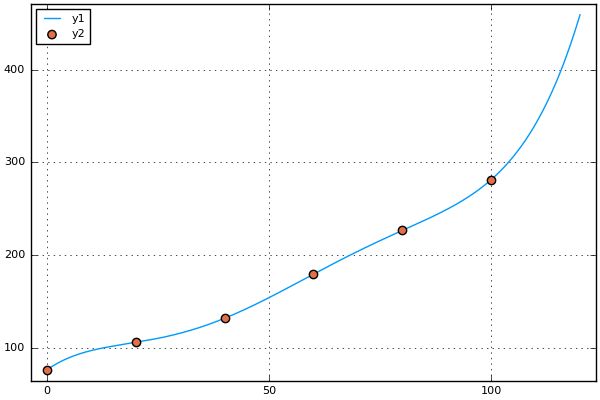
\includegraphics[width=\textwidth,keepaspectratio]{Problem1Images/interp.png}
\hfill \break
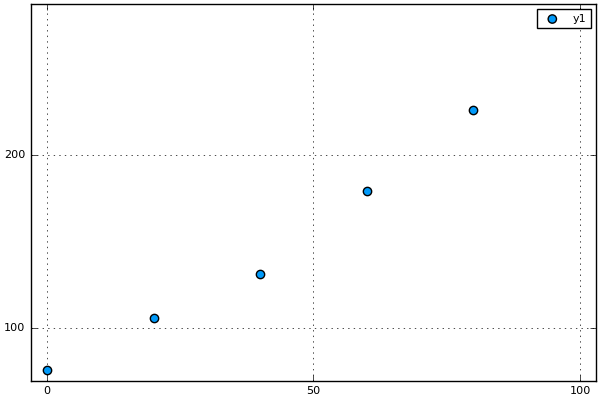
\includegraphics[width=\textwidth,keepaspectratio]{Problem1Images/scatter.png}
	\item
	\[p(x) = 76 \frac{(x-20)(x-40)}{(-20)(-40)} + 105.7 \frac{x(x-40)}{20(20-40)} + 131.7 \frac{x(x-20)}{40(40-20)} \]
\hfill \break
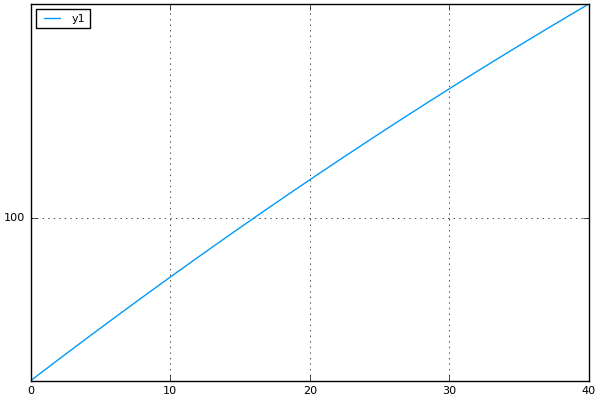
\includegraphics[width=\textwidth,keepaspectratio]{Problem1Images/lag.png}
	\end{enumerate}
\item
The Lagrange interpolant tends towards $-\infty$, and does not interpolate the data correctly at all. The Barycentric interpolant does correctly interpolate the data. 
\hfill \break
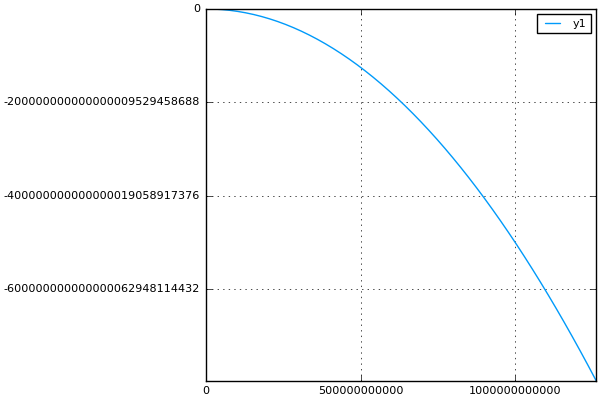
\includegraphics[width=\textwidth,keepaspectratio]{Problem1Images/lagms.png}
\hfill \break
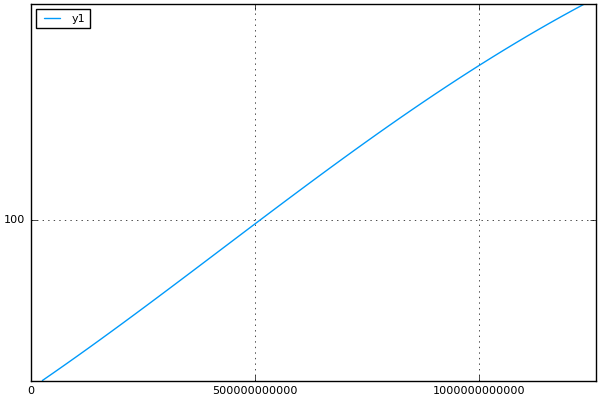
\includegraphics[width=\textwidth,keepaspectratio]{Problem1Images/mybary.png}
\item The reason this barycentric function is able to correctly interporlate the data, and not run into the same issues that Lagrange form had is that is forces the data to exact at the data points. Lagrange assumes that the calculation will force it to be so, but with floating point error this is not always the case. 
\hfill \break
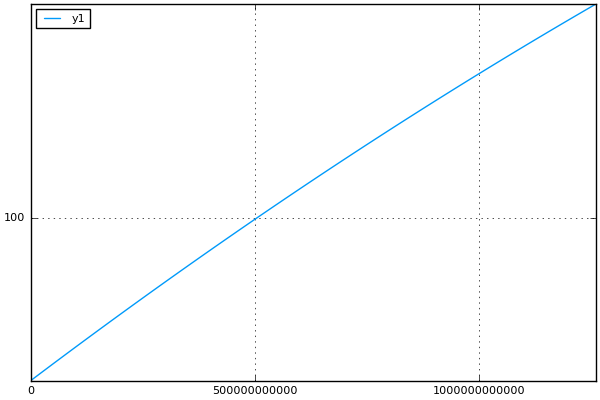
\includegraphics[width=\textwidth,keepaspectratio]{Problem1Images/baryfun.png}
\end{enumerate}
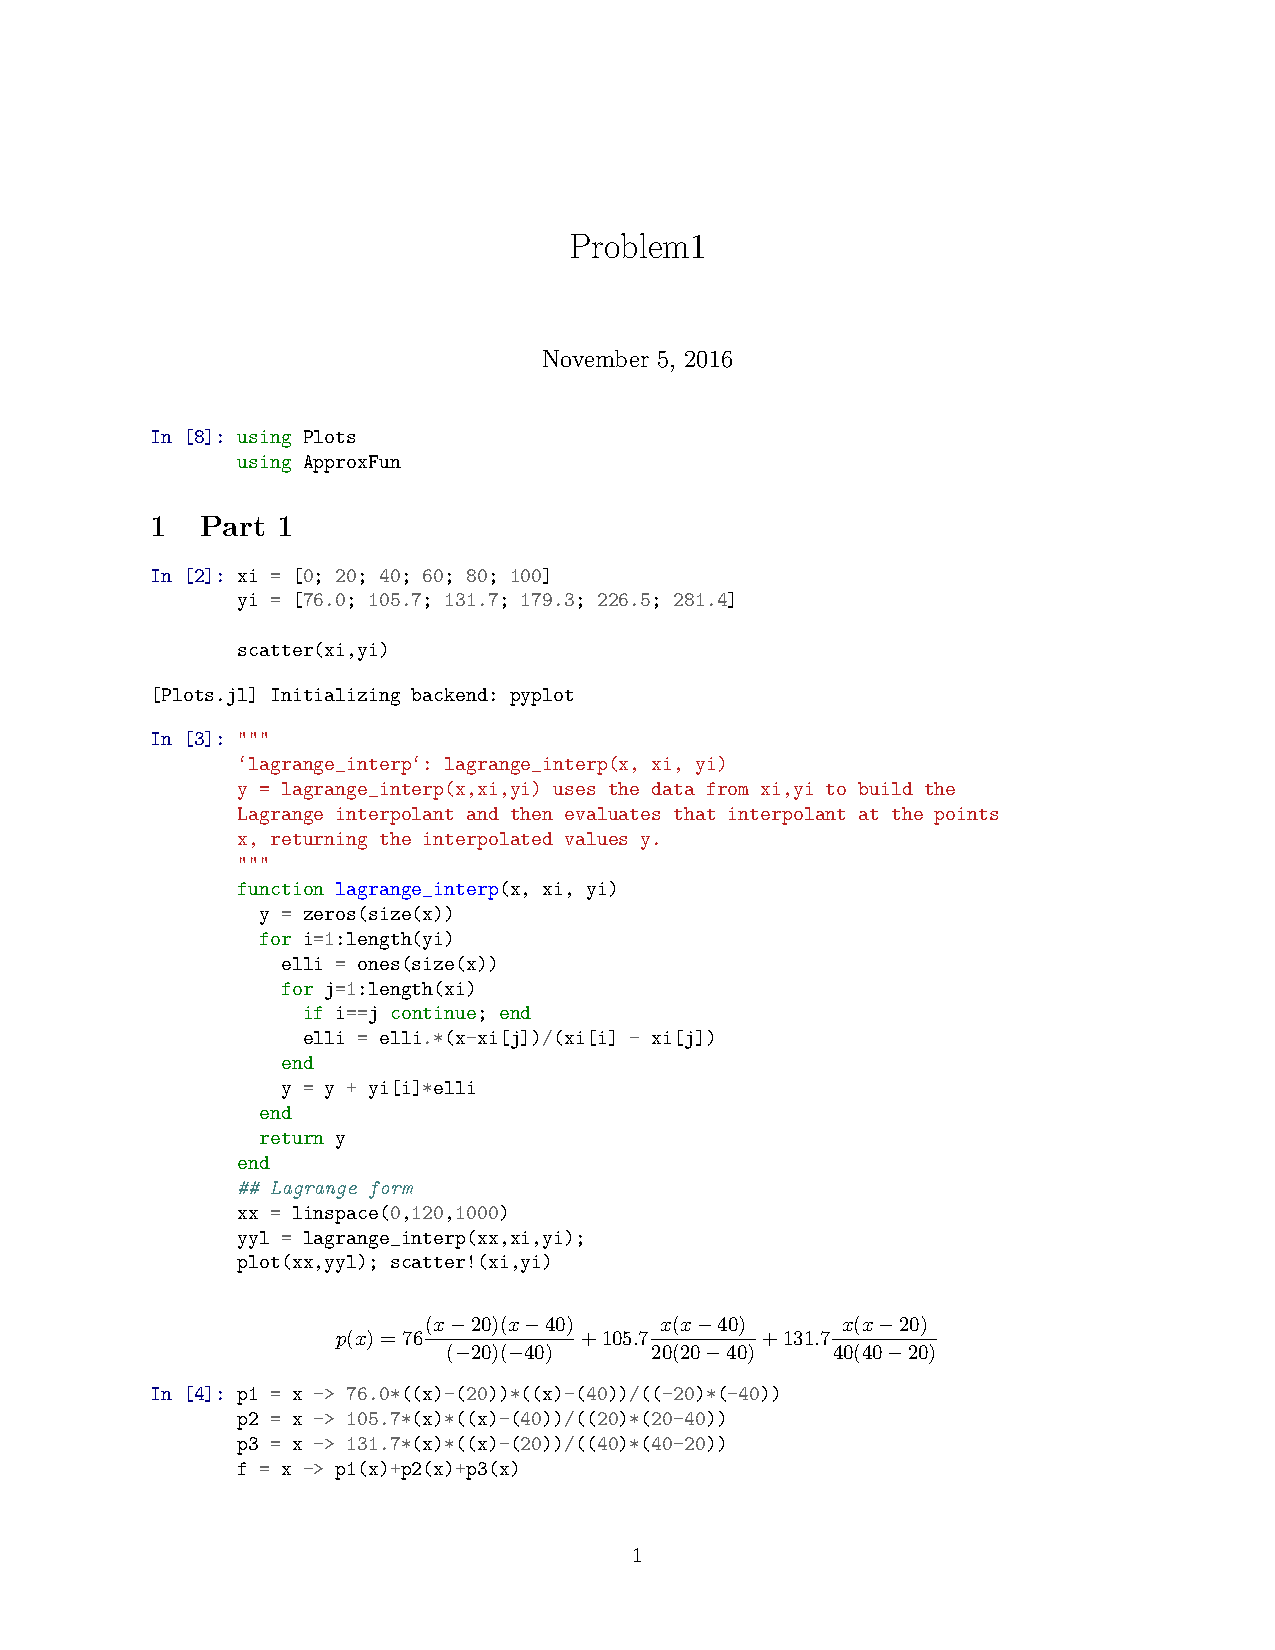
\includepdf[pages=-]{Problem1.pdf}

\subsection{Problem 2 (20 points)}\label{problem-2-20-points}

\begin{enumerate}
\def\labelenumi{\arabic{enumi}.}
\item
  Chapter 8, Problem 5.
\item
  Implement a Julia function that computes the following:

\begin{verbatim}
"""
`chebspace`
===========

A Chebyshev analog of linspace for polynomial interpolation

* `chebspace(a,b)` generates an array of 100 Chebyshev points 
between `a` and `b`
* `chebspace(a,b,n)` generates an array of `n` points between a, b
and for `n=1`, this returns b.
function chebspace(a,b,n)
# fill this in!
end
function chebspace(a,b)
    return chebspace(a,b,100)
end
\end{verbatim}

  (Hint, see equation 8.15)
\end{enumerate}

\subsection{Problem 2 Solution} %Solution start
\begin{enumerate}
\def\labelenumi{\arabic{enumi}.}
\item
$l(x) = -\frac{x-b}{a-b} + \frac{x-a}{b-a} $
\item
\end{enumerate}
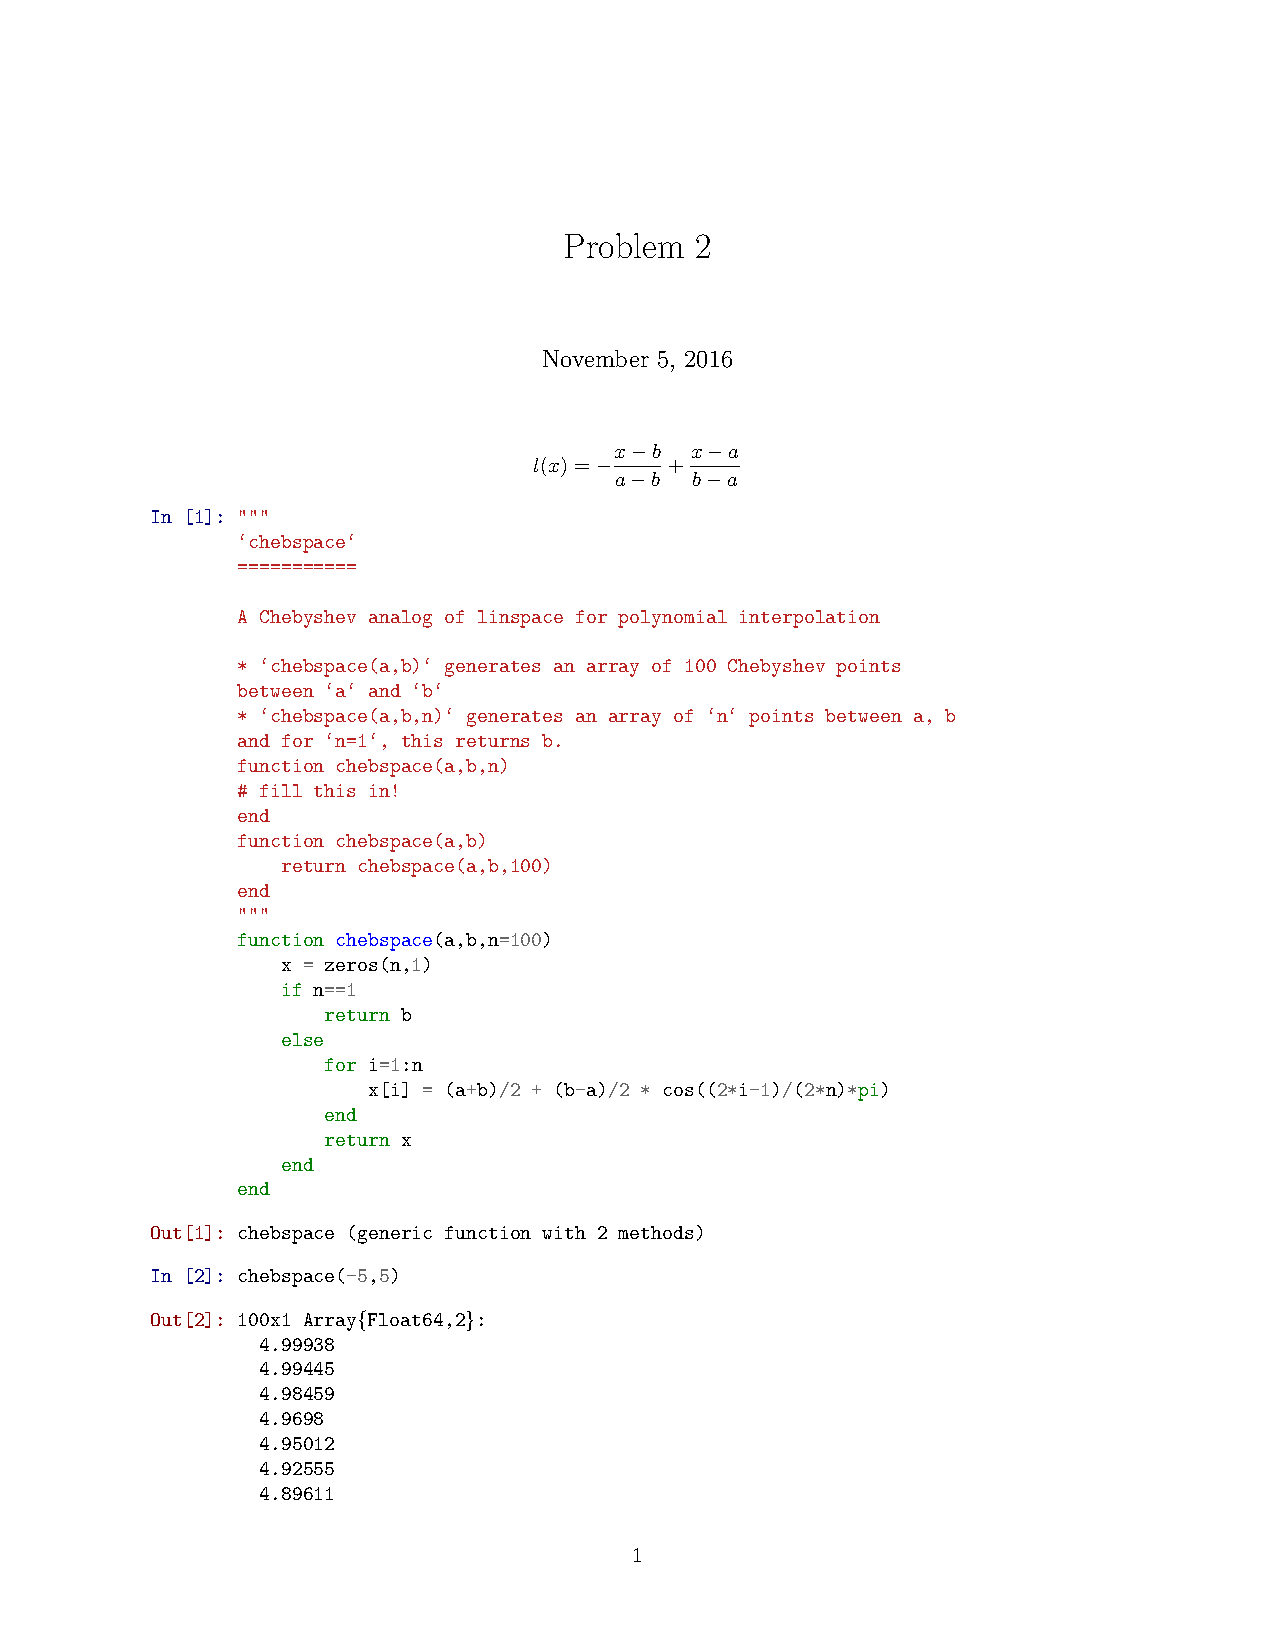
\includepdf[pages=-]{Problem2.pdf}

\subsection{Problem 3 (10 points)}\label{problem-3-10-points}

Write a paragraph or two (100-200 words) about what you learned about
polynomials and polynomial interpolation. You should also think about
answering the following questions:

\begin{enumerate}
\def\labelenumi{\arabic{enumi}.}
\itemsep1pt\parskip0pt\parsep0pt
\item
  Do you think you'd ever use polynomial interpolation?
\item
  If so, how?
\item
  If not, why not?
\end{enumerate}

Be honest, but remember to be thoughtful.

\subsection{Problem 3 Solution} %Solution start

\def\labelenumi{\arabic{enumi}.}
I do not think I will use polynomial interpolation too often. Most of the time it seems that approximation is more useful for visualization of data sets. The application of in typography is neat, but I do not think that I will ever be designing fonts. I suppose the main limitation I see with interpolation is that data sets are often chaotic, and fitting to everypoint does not give as good of a picture to an approximately correct graph. I would not say I will never use interpolation however, as there are often times when I need to plot a smooth function, and for this application interpolation makes sense. 



\subsection{Problem 4 (10 points)}\label{problem-4-10-points}

\begin{enumerate}
\def\labelenumi{\arabic{enumi}.}
\item
  Download and install ApproxFun. Then type \texttt{using ApproxFun} to
  get it added to your Julia instance. Also type \texttt{using Plots} to
  get the plotting interaface.
\item
  Run

\begin{verbatim}
f = Fun(x->sign(x))
plot(f)
\end{verbatim}

  How does this relate to the Weistrauss approximation theorem?
\item
  Try using ApproxFun to integrate the most complicated function (in one
  dimension) that you can think of! Can you stump ApproxFun?
\item
  One of the advantages of Chebfun is we can get computer
  representations of functions (as polynomials) that have no analytic
  form what-so-ever. Consider the following code which builds a
  polynomial approximation of
  \[ \rho(t) = \max |\lambda_i\left( t \bmat{1 & 2 & 0 \\ 0 & 2 & 1 \\ 1 & 0 & 2} + 
                      (1-t) \bmat{1 & 1 & 0 \\ 1 & -1 & 1 \\ -1 & 1 & 1} \right) | \]
  here $\lambda_i$ is just the $i$th eigenvalue. So this is looking at
  the largest magnitude eigenvalue. (Example from Chebfun:
  \url{http://www.chebfun.org/examples/approx/NoisyNonsmooth.html})

\begin{verbatim}
A = [1 2 0; 0 2 1; 1 0 2.0]
B = [1 1 0; 1 -1 1; -1 1 1.0]
f = Fun(t -> maximum(abs(eigvals(t*A + (1-t)*B))),[0,1])   
plot(f)
\end{verbatim}

  Run this code and show your result!
\item
  (Fun bonus question, worth no points.) This requires Matlab. Download
  and install the Matlab package \texttt{chebfun} Run
  \texttt{chebsnake('equi')} (Remember this when you are tempted to use
  equally spaced points for polynomial interpolation!)
\end{enumerate}

\subsection{Problem 4 Solution} %Solution start
\begin{enumerate}
\def\labelenumi{\arabic{enumi}.}
\item
\item
The theorem states that any continuous function can be approximated as closely as desired by a polynomial function. The sign function's plot reveals that it is challenging to have the maximum error approach 0, around the point $x=0$. 
\hfill \break
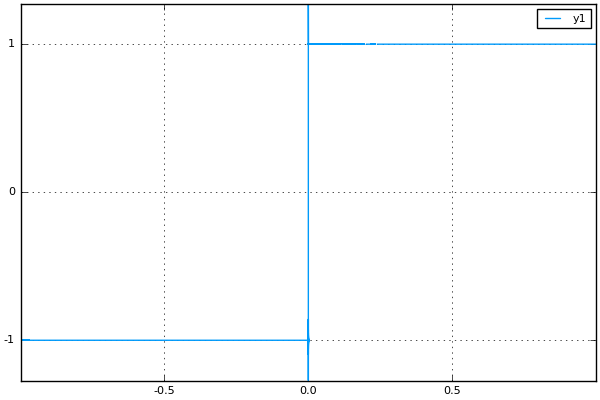
\includegraphics[width=\textwidth,keepaspectratio]{Problem4Images/problem4part2.png}
\item
\[ f(x) = sinh^{-1}(csc^2 (\frac{\pi * x }{e^x})) +2x \]
\hfill \break
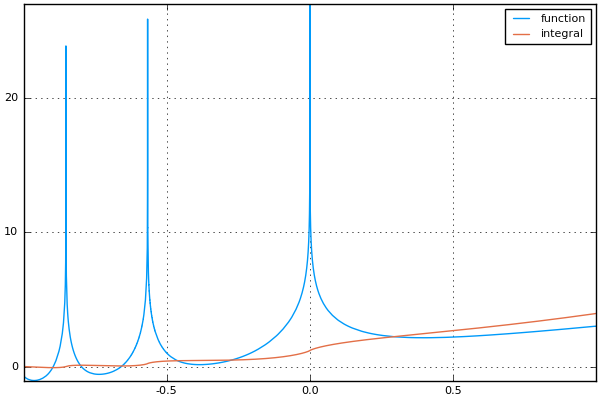
\includegraphics[width=\textwidth,keepaspectratio]{Problem4Images/problem4part3.png}
\item
\hfill \break
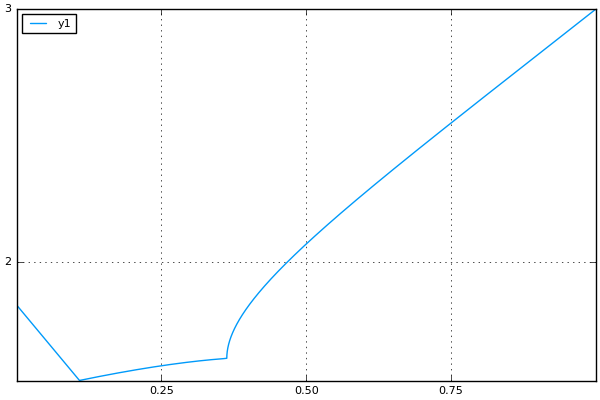
\includegraphics[width=\textwidth,keepaspectratio]{Problem4Images/problem4part4.png}
\item
\end{enumerate}
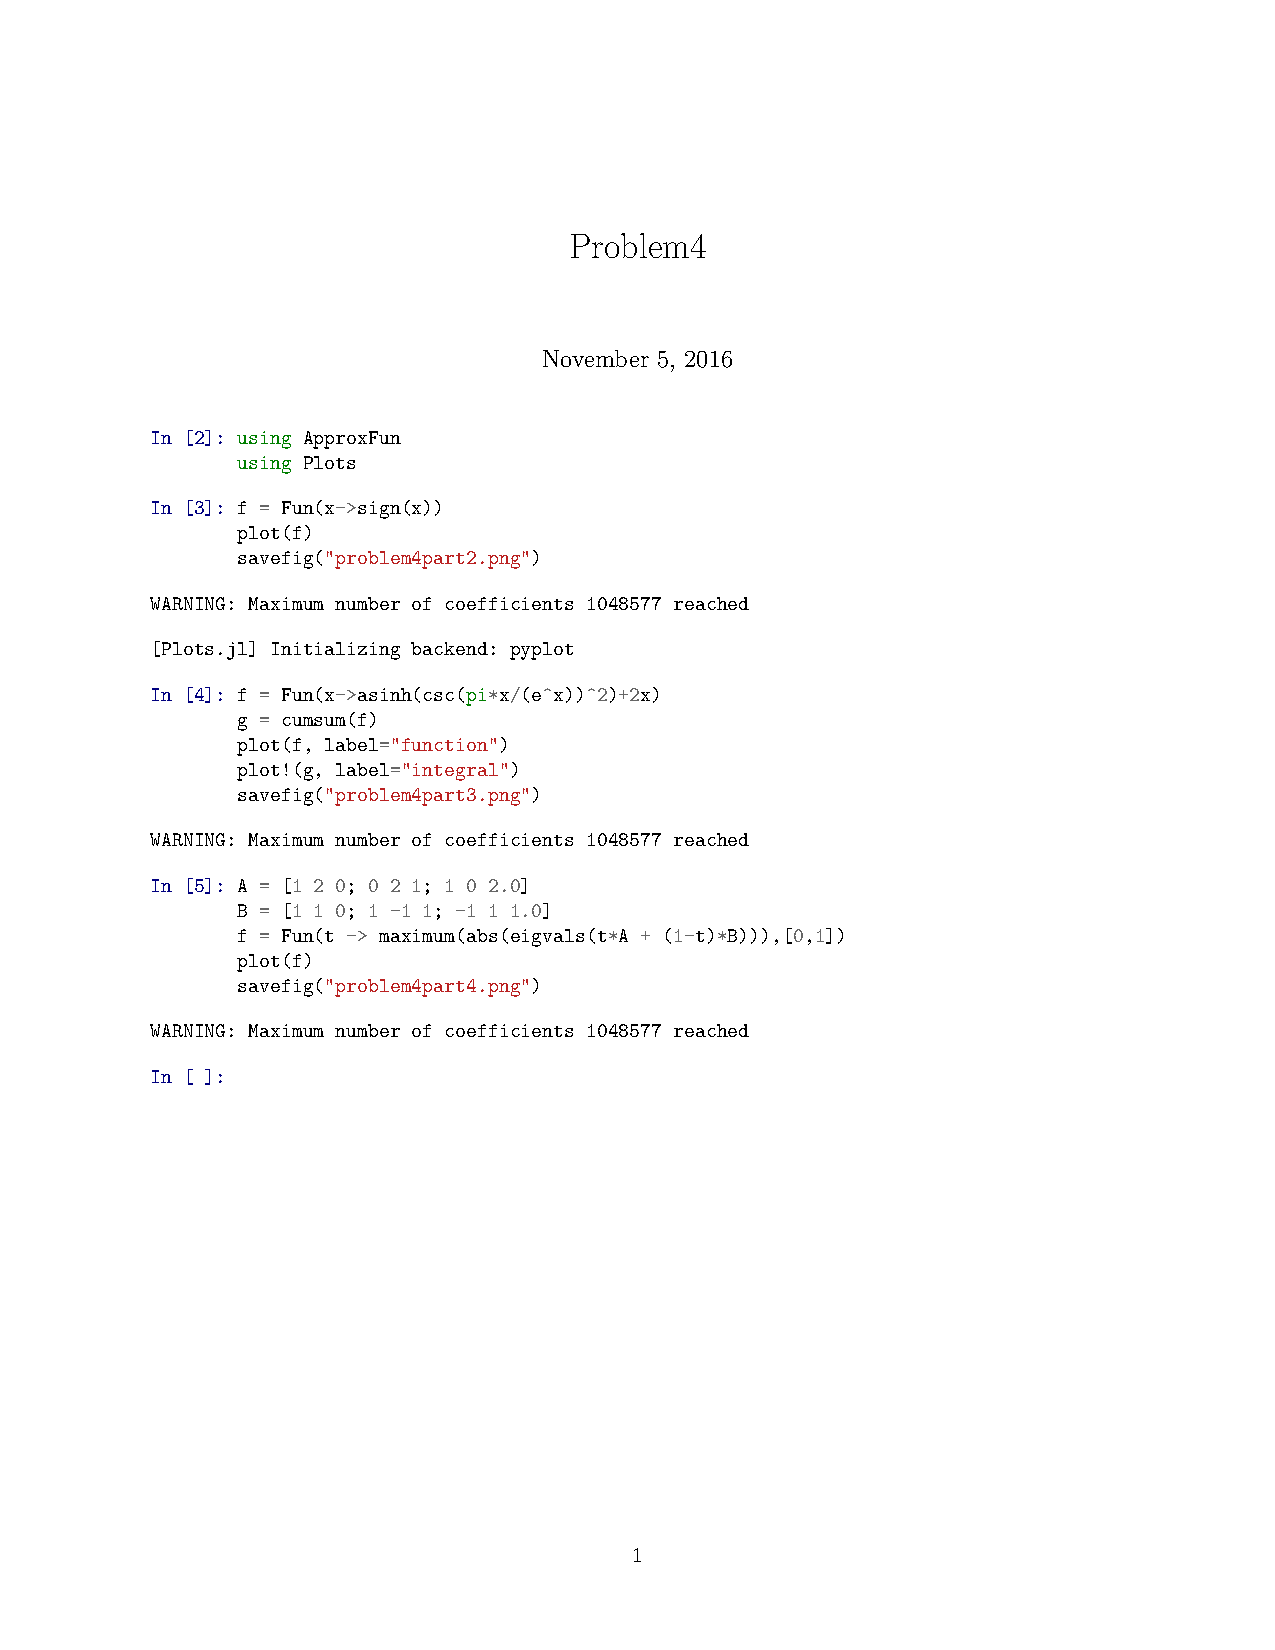
\includepdf[pages=-]{Problem4.pdf}


\subsection{Problem 5 (40 points)}\label{problem-5-40-points}

\begin{enumerate}
\def\labelenumi{\arabic{enumi}.}
\itemsep1pt\parskip0pt\parsep0pt
\item
  (10 points) Chapter 9, Exercise 1,
\item
  (10 points) Chapter 9, Exercise 2.
\item
  (10 points) Chapter 9, Exercise 3.
\item
  (10 points) Chapter 9, Exercise 5.
\end{enumerate}

\subsection{Problem 5 Solution} %Solution start
\begin{enumerate}
\def\labelenumi{\arabic{enumi}.}
\item
The lowest error was observed at $h=10^{-4}$. One reason for this is that the $h$ term in the denominator is squared, and as observed in central and forward difference, the optimal value is around $10^{-8}$ digits, so that would correspond to $h\approx 10^{-4}$
\item
It is obvious to see how much more quickly the error decreases in Richardson's compared to the previous approximation. For $h=0.2$ the erro was the same as $h=10^{-5}$. And for 2 steps of Richardson, the error was much smaller than the best of the previous analysis. 
\item
error is $1.14908e-14$
\item
\[f(x+h) = f(x) +hf'(x) + \frac{h^2}{2}f''(x) + \frac{h^3}{6}f'''(\eta) \]
\[f(x+2h)=f(x)+2hf'(x)+\frac{4h^2}{2}f''(x) + \frac{8h^3}{6}f'''(\xi)\]
\\
Multiply the top equation by 4, and the second by -1, then add the two. 
\[4[f(x+h) = f(x) +hf'(x) + \frac{h^2}{2}f''(x) + \frac{h^3}{6}f'''(\eta)] \]
\[-[f(x+2h)=f(x)+2hf'(x)+\frac{4h^2}{2}f''(x) + \frac{8h^3}{6}f'''(\xi)] \]
\\
\[4f(x+h)-f(x+2h) = 3f(x)+2hf'(x)+0 +\frac{2h^3}{3}(f'''(\eta)-f'''(\xi)) \]
Rearrange the terms to solve for $f'(x)$
\[f'(x) = \frac{1}{2h}[-3f(x)+4f(x+h)-f(x+2h)] + \frac{h^2}{3}(f'''(\eta)-f'''(\xi))\]
Therefore, the error term is $O(h^2)$
\end{enumerate}
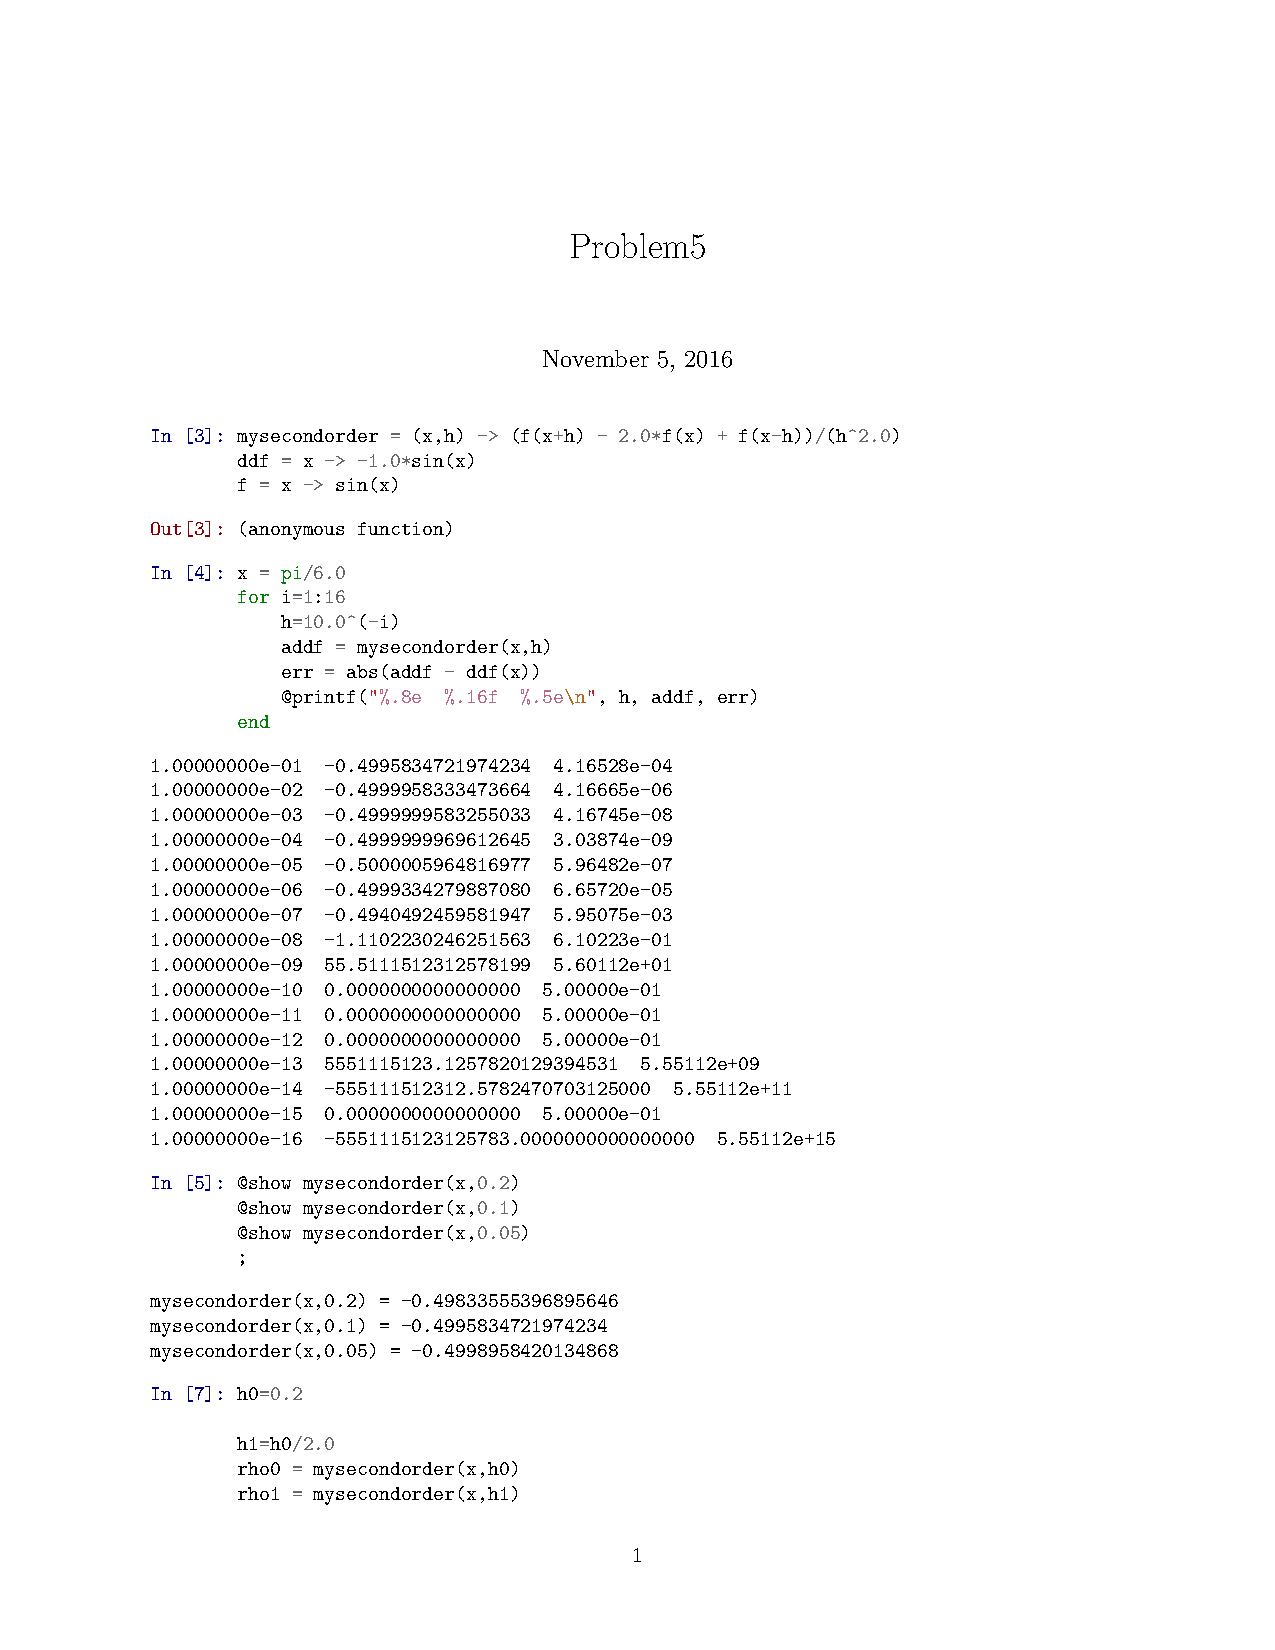
\includepdf[pages=-]{Problem5.pdf}


\end{document}
